\section{Arquitectura del sistema}

\subsection{Tecnologías seleccionadas}
\noindent Hoy en d\'ia, el ecosistema de herramientas y marcos de trabajo para el desarrollo web es muy amplio, abarcando desde bibliotecas para la interfaz de usuario hasta soluciones para el backend y la gesti\'on de tareas en segundo plano. A continuación se tienen diferentes tablas con algunas de las tecnologías mas destacadas para cada uno de los componentes que comprende la arquitectura el prototipo web.

\begin{table}[H]
\centering
\begin{tabular}{|l|p{10cm}|}
\hline
\textbf{Tecnología Frontend} & \textbf{Descripción} \\
\hline
Vue.js & Simplicidad y facilidad de integración, ideal para proyectos ligeros y rápidos de desarrollar. \\
\hline
Angular & Respaldado por Google, con una arquitectura robusta pensada para aplicaciones empresariales de gran escala. \\
\hline
Svelte & Enfoque innovador al compilar sus componentes en JavaScript puro, eliminando el uso del DOM virtual y logrando un mejor rendimiento. \\
\hline
React & Gran versatilidad, integración natural con TypeScript y Tailwind CSS. Arquitectura basada en componentes re-utilizables y escalables. \\
\hline
\end{tabular}
\caption{Tecnologías destacadas para el desarrollo frontend}
\end{table}

\noindent Con base en estas características, se seleccionó React como la tecnología más conveniente y eficiente para el desarrollo de la interfaz de usuario del prototipo.
\\
\\

\begin{table}[H]
\centering
\begin{tabular}{|l|p{10cm}|}
\hline
\textbf{Tecnología API Backend} & \textbf{Descripción} \\
\hline
Django & Conocido por su robustez, seguridad y rapidez de desarrollo. \\
\hline
Flask & Ideal para aplicaciones más pequeñas o que requieren mayor flexibilidad. \\
\hline
Node.js & Basado en JavaScript, permite usar un mismo lenguaje tanto en el frontend como en el backend, promoviendo la uniformidad en el desarrollo. \\
\hline
FastAPI & Ligero y eficiente. Utiliza tipado estático para mejorar la claridad y documentación de las APIs, facilitando la integración con servicios externos.\\
\hline
\end{tabular}
\caption{Tecnologías destacadas para el desarrollo backend}
\end{table}

\noindent Por su eficiencia, facilidad de uso y moderna arquitectura, FastAPI fue seleccionada como la opción ideal para el desarrollo del backend del prototipo.
\\
\\
En el desarrollo de aplicaciones web modernas, contar con un sistema para la gestión de tareas en segundo plano resulta  beneficioso, especialmente cuando se ejecutan procesos intensivos como aquellos relacionados con modelos de inteligencia artificial. Este tipo de soluciones permite liberar al servidor principal de operaciones pesadas, lo cual evita bloqueos o lentitud en la atención de las solicitudes y garantiza una experiencia de usuario más fluida y eficiente. En el caso del presente proyecto, esta necesidad se vuelve aún más relevante al momento de generar lecciones que requieren procesamiento con modelos de IA, lo cual podría afectar negativamente el rendimiento general del sistema. 
\begin{table}[H]
\centering
\begin{tabular}{|l|p{10cm}|}
\hline
\textbf{Tecnología } & \textbf{Descripción} \\
\hline
RQ & Herramienta sencilla para gestionar tareas en segundo plano utilizando Redis como sistema de cola. \\
\hline
Dramatiq & Sistema de colas basado en Python, conocido por su buen rendimiento y facilidad de uso. \\
\hline
Celery & Herramienta madura, compatible con distintos brokers de mensajes y altamente configurable. Se pueden programar tareas periódicas (Celery Beat). \\
\hline
\end{tabular}
\caption{Tecnologías destacadas para la gestión de tareas en segundo plano}

\end{table}

\noindent Dado el contexto del proyecto y la necesidad de procesar tareas intensivas como la generación de lecciones con modelos de IA, se eligió Celery junto con Celery Beat por su robustez y flexibilidad.
\\
\\
En lo que respecta a la gestión de bases de datos dentro del desarrollo del prototipo, se optó por utilizar PostgreSQL y Redis. Esta elección se basa principalmente en la familiaridad previa con estas herramientas, así como en el hecho de que la lógica de integración y manipulación de datos no difiere significativamente entre tecnologías similares, lo que permite enfocar los esfuerzos en otros aspectos más críticos del sistema.

\begin{table}[H]
\centering
\begin{tabular}{|p{3cm}|p{9cm}|}
\hline
\textbf{Tecnología} & \textbf{Descripción} \\
\hline
PostgreSQL & Sistema de gestión de bases de datos relacional, conocido por su estabilidad, conformidad con estándares SQL y capacidades avanzadas como el manejo de tipos de datos complejos y extensiones. \\
\hline
Redis & Almacén de datos en memoria, basado en estructuras clave-valor, ideal para operaciones rápidas y uso como sistema de caché o base de datos secundaria para tareas de alta concurrencia. \\
\hline
\end{tabular}
\caption{Tecnologías utilizadas para la gestión de bases de datos}
\end{table}


Teniendo en cuenta lo anterior se presentan las tecnologías seleccionadas para cada componente de la arquitectura.


\begin{itemize}
    \item \textbf{Frontend:} Implementado con React, TypeScript y Tailwind CSS. Este componente se encarga de la interfaz de usuario, permitiendo la interacci\'on del usuario con las lecciones, preguntas y resultados.
    
    \item \textbf{Backend (API):} Utiliza FastAPI para gestionar las peticiones provenientes del frontend. Este servidor maneja la autenticación, el enrutamiento y la comunicación con la base de datos, así como con los servicios asíncronos. Internamente, sigue una arquitectura basada en el patrón Modelo-Vista-Controlador (MVC).
    
    \item \textbf{Gestión de tareas (as\'incrono):} Se apoya en Celery y Celery Beat para procesar tareas de forma peri\'odica. Este servicio trabaja de forma desacoplada del servidor principal, permitiendo la escalabilidad del sistema.

    \item \textbf{Base de datos NoSQL:} Redis sirve como sistema de almacenamiento en memoria para consultas r\'apidas, evitando el acceso constante a la base de datos. Ademas, Redis se utiliza como el brocker y backend para la cola de tareas en celery, siendo en el index 0 broker y en el indice 1 backend (es decir, donde guarda los estados de las tareas y sus resultados).

    \item \textbf{Base de datos SQL:} Se utiliza PostgreSQL alojado en NeonDB. Esta base de datos almacena toda la informaci\'on relevante del sistema, incluyendo usuarios, rachas, lecciones y preguntas incorrectas.
\end{itemize}

\noindent Esta arquitectura permite una separaci\'on clara de responsabilidades, facilita la escalabilidad del sistema distribuye las cargas entre procesos sincr\'onos y as\'incronos.



\newpage
\section{Explicación del prototipo.}

Antes de profundizar en los detalles del funcionamiento del prototipo, es fundamental presentar su estructura lógica general.
\\
\\
El prototipo está centrado exclusivamente en la entidad usuario, quien es el único actor que interactúa directamente con el sistema. Una vez que accede a la plataforma, el usuario puede visualizar y participar en diversas lecciones, las cuales están compuestas por un conjunto de preguntas.
\\
\\
Cada lección se organiza de forma estructurada, incluyendo un texto base que introduce el tema de la lección, seguido de dos preguntas. Cada pregunta está acompañada por su respuesta correcta y una incorrecta, lo cual permite evaluar la comprensión del usuario.

\section{Diseño de base de datos}
\noindent La base de datos relacional para el prototipo tiene como objetivo central gestionar la información relacionada con los usuarios y su proceso de aprendizaje a través de lecciones y preguntas (dicho proceso se explica a mas detalle en el capitulo 6). Para ello, se estructura en seis (6) tablas principales: \textbf{usuarios}, \textbf{lecciones}, \textbf{preguntas}, \textbf{registro\_preguntas}, \textbf{lecciones\_resueltas} y \textbf{rachas}. Cada una de estas tablas cumple una función específica dentro del sistema y se encuentra relacionada para facilitar el acceso eficiente y coherente a los datos.
\\
\\
A continuación se presenta una descripción breve de cada tabla:
\begin{itemize}
  \item \textbf{usuarios}: almacena la información principal de cada usuario del sistema.
  \item \textbf{lecciones}: contiene los registros de las lecciones generadas, incluyendo su contenido.
  \item \textbf{preguntas}: guarda el contenido de las preguntas asociadas a cada lección.
  \item \textbf{registro\_preguntas}: almacena el resultado de las preguntas que el usuario ha respondido, permitiendo realizar un seguimiento de las preguntas respondidas incorrectamente para reutilizarlas en la sección de preguntas incorrectas del prototipo.
  \item \textbf{lecciones\_resueltas}: registra todas las lecciones que el usuario ya ha completado.
  \item \textbf{rachas}: controla elementos de gamificación, como la cantidad de días consecutivos en los que un usuario ha respondido correctamente al menos una pregunta y la experiencia global obtenida.
\end{itemize}

\subsection{Modelo Entidad Relación }

\begin{figure}[H]
  \centering
  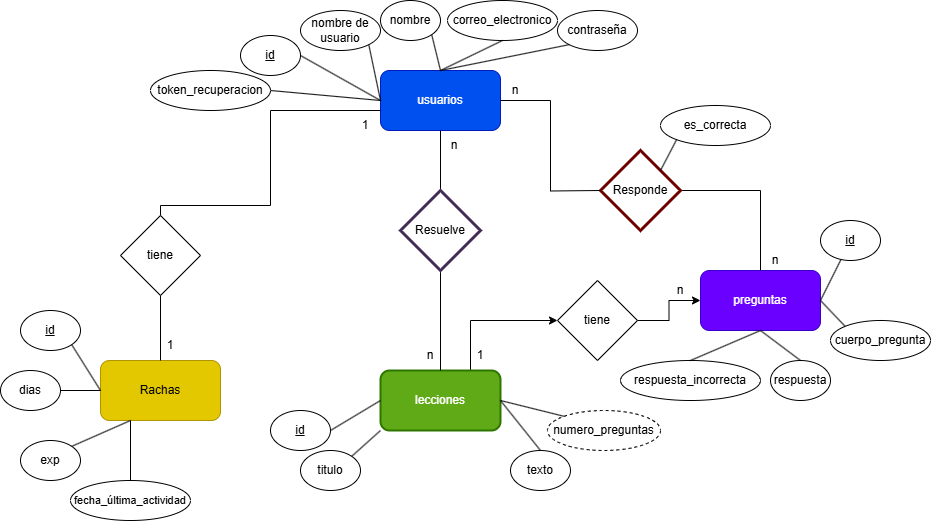
\includegraphics[width=0.9\linewidth]{Imagenes/DB_RM.png}
  \caption{Modelo Entidad Relación}
  \label{fig:ER}
\end{figure}


\subsection{Modelo UML}

\begin{figure}[H]
  \centering
  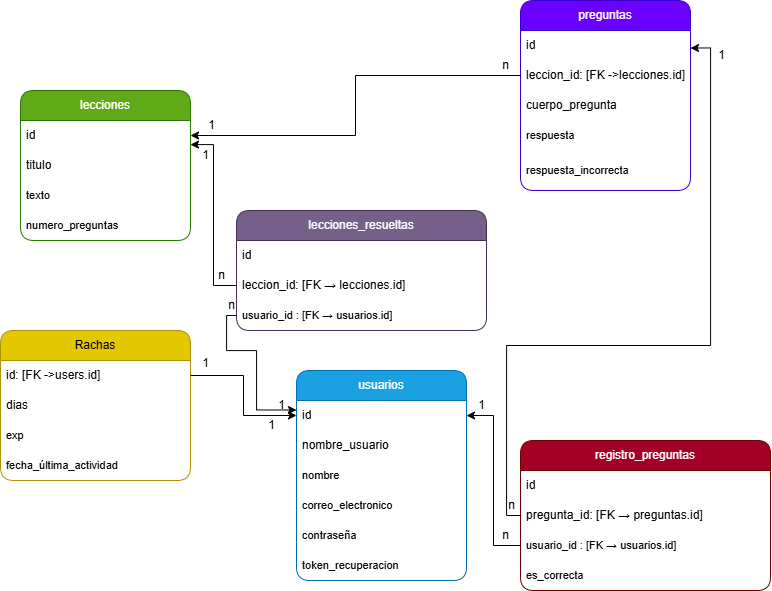
\includegraphics[width=0.6\linewidth]{Imagenes/DB_UML.png}
  \caption{Modelo UML}
  \label{fig:uml}
\end{figure}


\subsection{Base de datos NoSQL}

A diferencia de las bases de datos relacionales, Redis, al ser una base de datos NoSQL (Not Only SQL) no utiliza un esquema estructurado predefinido, ya que se basa en el almacenamiento de datos en formato clave-valor. Por esta razón, a continuación se detalla las claves utilizadas, los tipos de datos asociados y una breve descripción de su propósito dentro del sistema. Esta representación permite comprender la lógica de almacenamiento empleada en Redis y su papel en el prototipo.

\begin{table}[H]
\centering
\begin{tabular}{|p{3.5cm}|l|p{6cm}|}
\hline
\textbf{Tipo} & \textbf{Nombre de la variable} & \textbf{Descripci\'on} \\
\hline
Hash & \texttt{lesson:\{lesson\_id\}} & Almacena atributos de la lecci\'on: ID, t\'itulo y cantidad de preguntas. Esto con el objetivo de brindar en la pagina principal del prototipo una breve descripcion de todas las lecciones recientes. \\
\hline
Conjunto (set) & \texttt{all\_lessons} & Contiene todas las claves de lecciones creadas recientemente. Se utiliza para acceder a todas las lecciones actuales de forma eficiente. \\
\hline
Conjunto (set) & \texttt{user:\{user\_id\}:completed} & Guarda los ID de las lecciones completadas por un usuario espec\'ifico. Facilita brindar al usuario solo las lecciones actuales que tiene pendientes por realizar. \\
\hline
\end{tabular}
\caption{Estructuras de datos utilizadas en Redis}
\label{table:EstructurasRedis}
\end{table}


\section{Interfaz de usuario (UI/UX)}

En esta sección se describe la interfaz de usuario en su diseño de mockups desarrolladas para la aplicación, las cuales fueron diseñadas utilizando la herramienta Figma. Durante el proceso de diseño se priorizó la experiencia del usuario, asegurando una navegación intuitiva y una estética coherente con los objetivos de la plataforma. Además, se implementó un enfoque responsive que permite que la interfaz se adapte adecuadamente a distintos tamaños de pantalla, garantizando una visualización óptima en dispositivos móviles, tabletas y computadoras de escritorio. A continuación, se detallan las principales secciones y componentes de la interfaz. Cabe resaltar que este no representa el diseño final de la aplicación, ya que siempre existe un margen de mejora y ajustes según la retroalimentación de los usuarios. Si desea ver todas las mockups del prototipo y su diseño final, dirigirse a los \hyperref[Anexos]{Anexos}.

\newpage
\subsubsection{Imágenes utilizadas}

Las imágenes utilizadas en este proyecto, incluyendo las insignias y la imagen de inicio de sesión, fueron generadas mediante la inteligencia artificial DALL·E de OpenAI. Según la política de contenido de OpenAI \cite{openaicondicionesuso}, los usuarios poseen los derechos sobre las imágenes que crean, incluyendo el derecho a reimprimir, vender y comercializar dichas imágenes, independientemente de si fueron generadas mediante créditos gratuitos o pagos. Por lo cual las imágenes utilizadas en la interfaz no tendrán problema por derechos de autor.

\begin{figure}[H]
  \centering
  
\includegraphics[width=0.8\linewidth]{Imagenes/Imagenes IA.png}
  \caption{Imágenes utilizadas}
  \label{fig:ER}
\end{figure}

\subsubsection{Módulo de logIn}

Este módulo permite el acceso de los usuarios que ya están registrados en el prototipo mediante correo electrónico y contraseña. La interfaz presenta un formulario simple, con campos identificados para el ingreso de credenciales. Además, se incluyen enlaces a las secciones “¿Olvidaste tu contraseña?” y “Regístrate”, que permiten respectivamente recuperar el acceso en caso de olvido y crear una nueva cuenta

\begin{figure}[H]
  \centering
  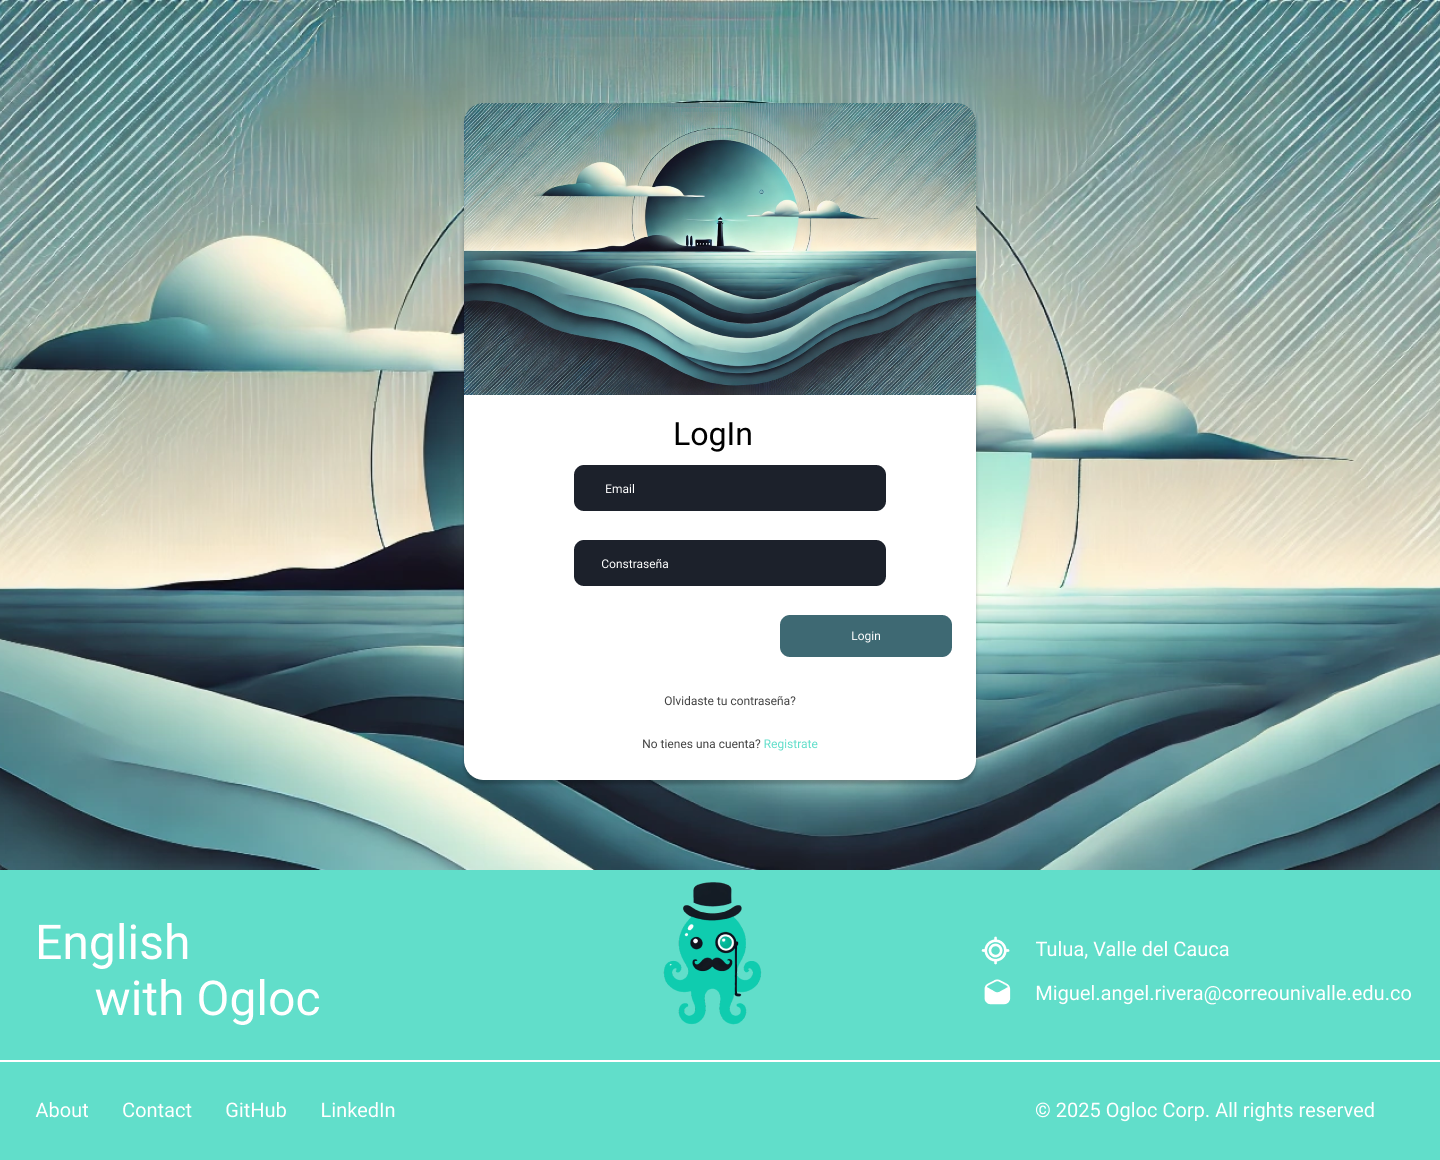
\includegraphics[width=0.8\linewidth]{Imagenes/Vista login.png}
  \caption{Mockup LogIn}
  \label{fig:ER}
\end{figure}

\subsubsection{Módulo de Registro}

El módulo de registro permite a los nuevos usuarios crear una cuenta en el prototipo mediante un formulario sencillo y accesible. Este formulario está compuesto por los campos: nombre completo, nombre de usuario (username), correo electrónico y contraseña. Cada uno de estos campos está diseñado para facilitar el ingreso de datos de manera clara y eficiente. Asimismo, se implementan validaciones básicas para asegurar que la información ingresada sea válida y coherente.

\begin{figure}[H]
  \centering
  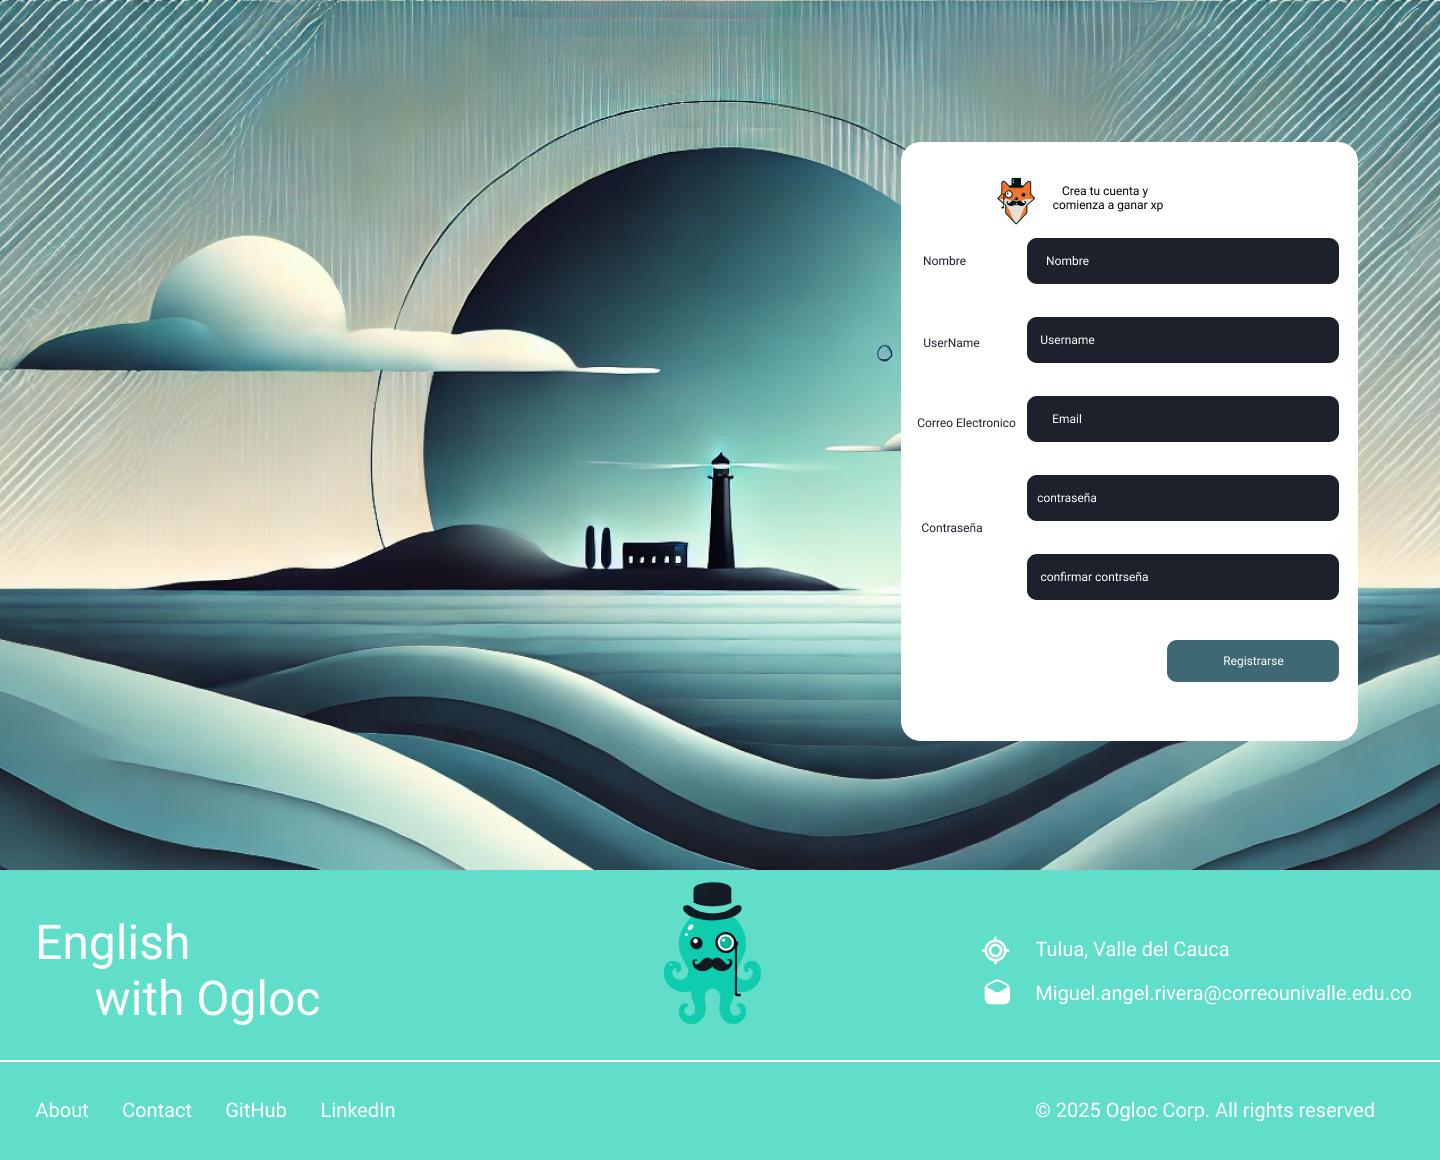
\includegraphics[width=0.6\linewidth]{Imagenes/Vista Registro.png}
  \caption{Mockup de Registro}
  \label{fig:ER}
\end{figure}


\subsubsection{Módulo perfil de usuario}

Este módulo permite al usuario visualizar y gestionar la información asociada a su cuenta. Desde esta sección, el usuario puede consultar datos como su nombre, nombre de usuario y su progreso dentro de la plataforma. Además, se incluye la posibilidad de editar algunos de estos datos o acceder a opciones adicionales como eliminar la cuenta.

\begin{figure}[H]
  \centering
  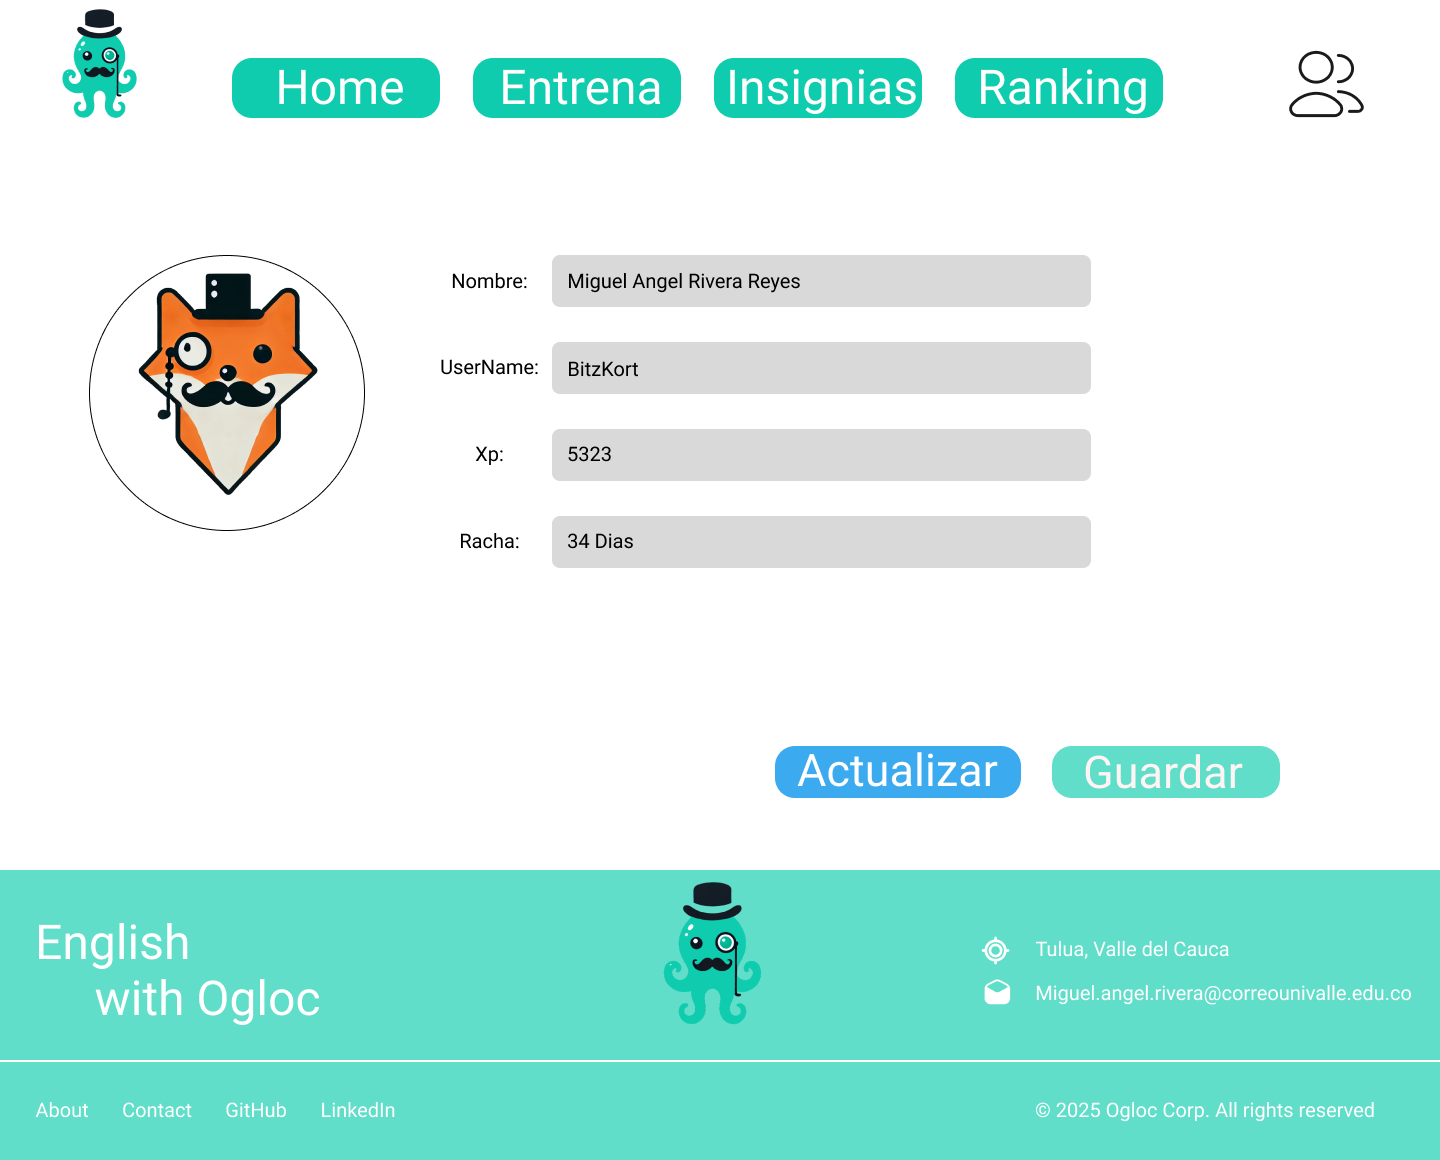
\includegraphics[width=0.5\linewidth]{Imagenes/vista perfil.png}
  \caption{Mockup perfil de usuario}
  \label{fig:ER}
\end{figure}

\subsubsection{Módulo preguntas}

Este módulo corresponde a la vista en la que se presentan las preguntas de cada lección , el usuario interactúa directamente con el contenido de aprendizaje respondiendo las preguntas que conforman una lección por medio del micrófono. Las preguntas se muestran una a una, de forma clara y ordenada.

\begin{figure}[H]
  \centering
  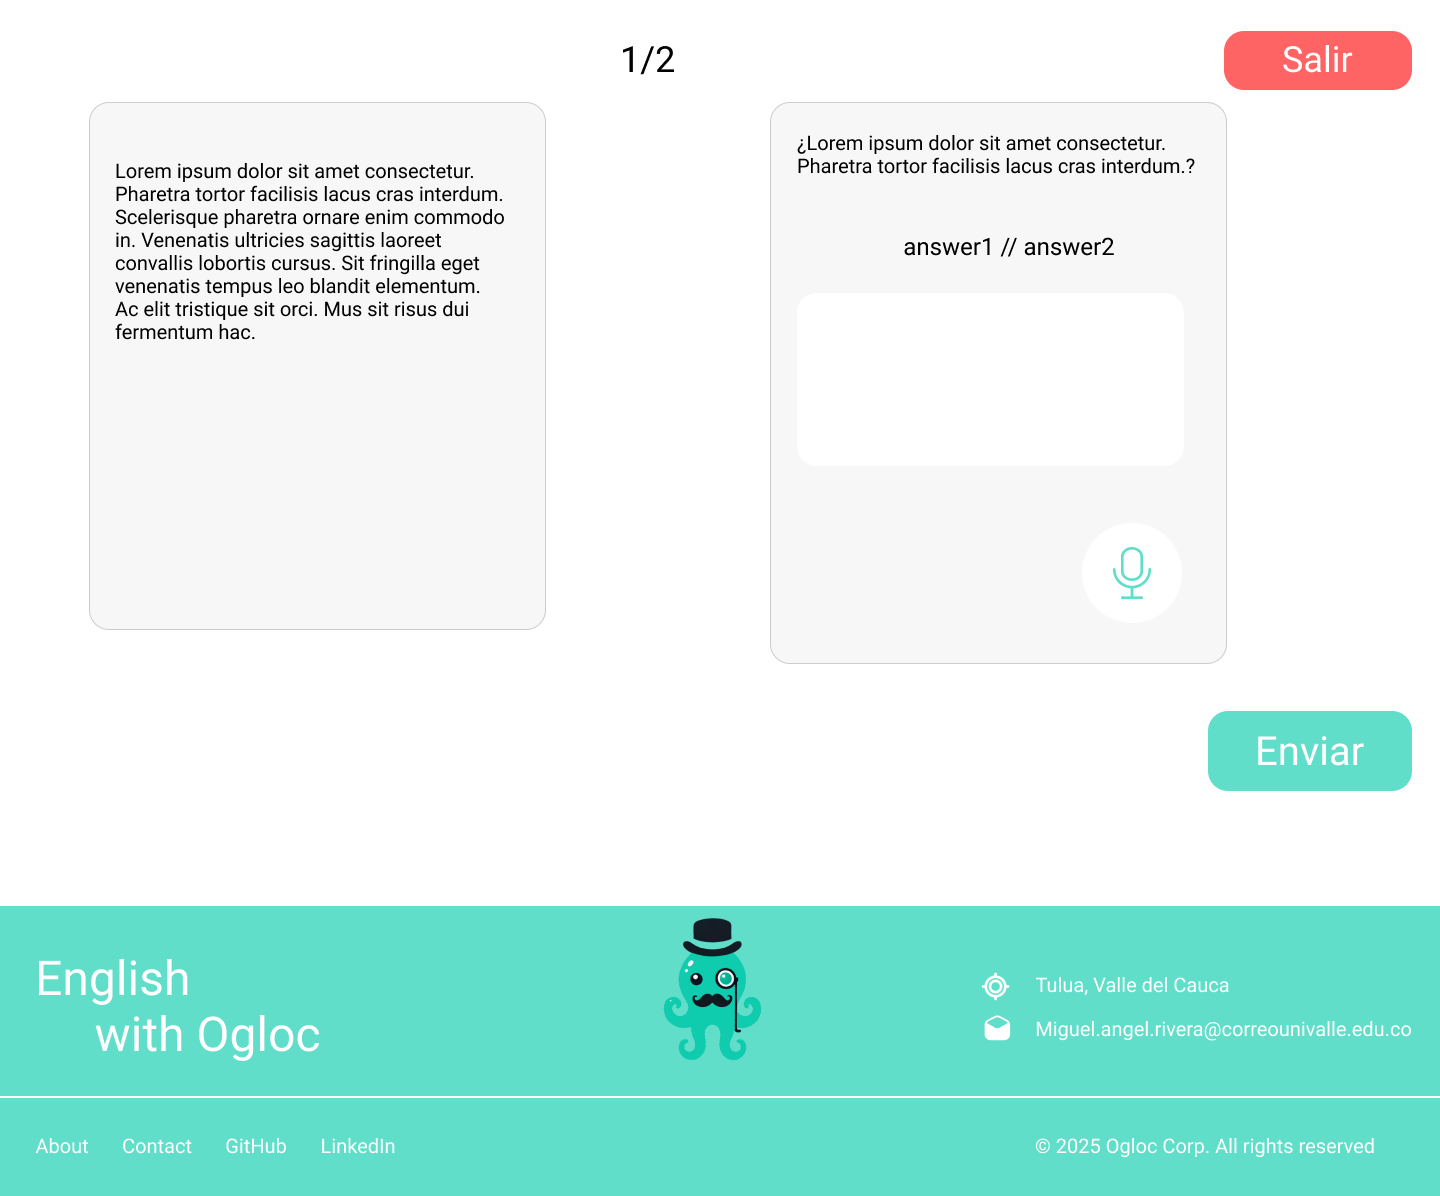
\includegraphics[width=0.6\linewidth]{Imagenes/Vista preguntas.png}
  \caption{Mockup vista preguntas}
  \label{fig:ER}
\end{figure}

\subsubsection{Módulo principal (home)}

Este módulo representa la página principal del prototipo, donde el usuario puede visualizar de forma general las funcionalidades más relevantes de la aplicación. En esta vista se presentan las lecciones disponibles para realizar, organizadas de manera que faciliten su acceso y comprensión. Además, se incluyen secciones dedicadas a las insignias obtenidas por el usuario, así como un acceso al pool de preguntas incorrectas, lo que permite reforzar los conocimientos previamente evaluados. Finalmente, se muestra un ranking global con los usuarios que han acumulado mayor experiencia (exp), promoviendo la motivación y el sentido de competencia entre los participantes.


\begin{figure}[H]
  \centering
  \includegraphics[width=0.5\linewidth]{Imagenes/Vista home.png}
  \caption{Mockup home}
  \label{fig:ER}
\end{figure}

\newpage
\subsubsection{Módulo Insignias}

Este módulo está dedicado a la visualización de las insignias que el usuario ha obtenido a lo largo de su progreso en la plataforma. Las insignias se otorgan en función de la cantidad de experiencia (exp) acumulada, la cual se incrementa a medida que el usuario responde correctamente las preguntas de las lecciones. Este sistema de recompensas tiene como objetivo incentivar la participación constante y reconocer el esfuerzo del usuario, proporcionando una representación visual de sus logros dentro de la aplicación. Las insignias se muestran de manera ordenada, permitiendo identificar tanto las obtenidas como las que aún están por desbloquear.

\begin{figure}[H]
  \centering
  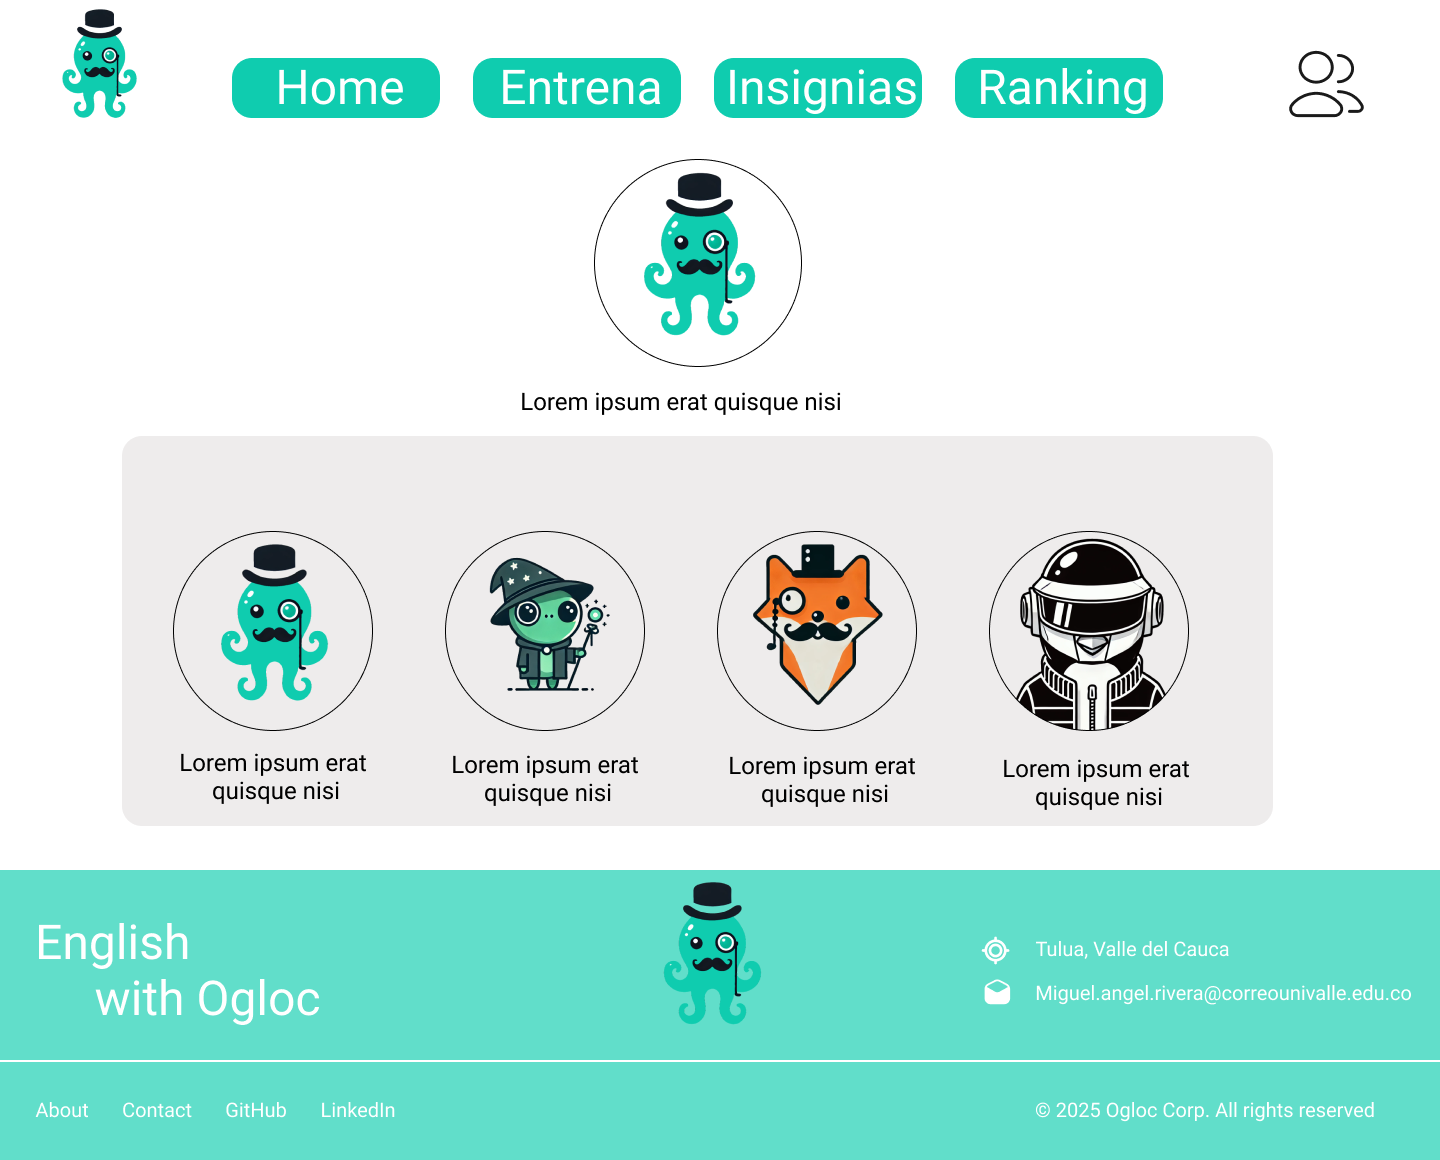
\includegraphics[width=0.6\linewidth]{Imagenes/Vista insignias.png}
  \caption{Mockup vista Insignias}
  \label{fig:ER}
\end{figure}

\newpage
\section{Diagrama de despliegue}

En el siguiente diagrama de arquitectura o de despliegue, se pueden visualizar los diferentes componentes que comprende la arquitectura del sistema. El diagrama es una herramienta que se utiliza para demostrar como están distribuidos los componentes de software en los diferentes elementos de hardware de un sistema.

\begin{figure}[H]
  \centering
  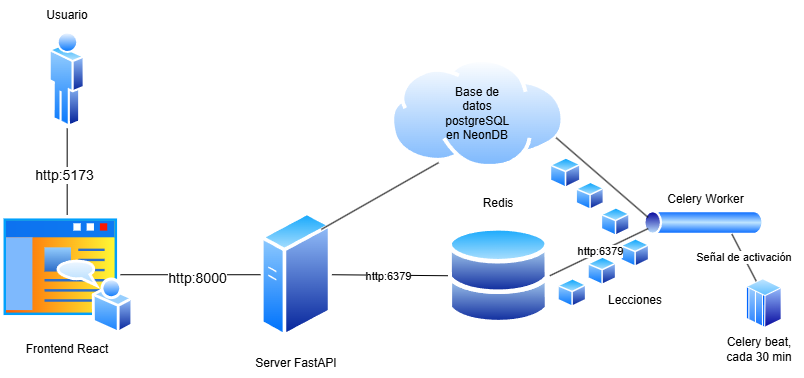
\includegraphics[width=0.9\linewidth]{Imagenes/Diagrama de despliegue.png}
  \caption{Diagrama de despliegue}
  \label{fig:ER}
\end{figure}